\documentclass[11pt]{article}
\input{preamble.tex}
\usepackage[left=1.5cm, right=1.5cm, top=1.3cm, includehead, includefoot]{geometry}

% Section labling for equations
\numberwithin{equation}{section}

%% Header
\pagestyle{fancy}
\fancyhead[L]{\bf\large Coxeter Group}
\fancyhead[R]{\bf\large Edward}
% \fancyfoot[C]{Page \thepage\ of 2}
\renewcommand{\headrulewidth}{0.4pt}
\renewcommand{\footrulewidth}{0.4pt}
\setlength{\headheight}{35pt}

% =====================================================================================================

\begin{document}
% =====================================================================================================
% Title page
\begin{titlepage}
  \begin{center}
    \vspace*{4cm}
    \textbf{\Huge{DRP F26 - Coxeter Group}}
 
    \vspace{1.5cm}
    Note Taker: \textbf{Edward Chang}

    Email: \textit{edward.chang@uwaterloo.ca}

    Updated: \today
  \end{center}
\end{titlepage}

\tableofcontents
\newpage
% =====================================================================================================
2026-09-14
\section{Introduction}
\begin{defm}{Group}
  A \textbf{group} \((G, \bullet)\) where \(G\) is a set and \(\bullet: G \times G \to G\) is a binary operator on the set, and it follows that:
  \begin{enumerate}[label=\roman*)]
    \item (Associativity): \(\forall a, b, c \in G, (a \bullet b) \bullet c = a \bullet (b \bullet c)\)
    \item (Identity element): \(\exists 1 \in G: \forall a \in G a \bullet 1 = 1 \bullet a = a\)
    \item (Inverse element): \(\forall a \in G \exists a ^{-1} \in G: a \bullet a ^{-1} = a ^{-1} \bullet a = 1\)
  \end{enumerate}
\end{defm}

\begin{center}
  \begin{tikzpicture}[scale=1.5, >=stealth]
    % Draw dashed rays for the remaining hyperplanes
    \foreach \angle in {90, 135, 180, 225, 270, 315} {
        \draw[dashed] (0,0) -- (\angle:1.5);
    }

    % Draw solid rays for primary mirrors a and b
    \draw[thick] (0,0) -- (0:1.5) node[right] {$a$};
    \draw[thick] (0,0) -- (45:1.5) node[above right] {$b$};

    % Angle theta between a and b
    \draw[thick] (0.6,0) arc (0:45:0.6) node[midway, left] {$\theta$};

    % The single star object in the fundamental domain

    % Reflection arrow Ra (across mirror a)
    \draw[<-, thick] (1.75, -0.35) to[bend right=45] node[right] {$R_a$} (1.75, 0.35);

    % Reflection arrow Rb (across mirror b)
    \draw[->, thick, rotate=45] (1.75, -0.35) to[bend right=45] node[right] {$R_b$} (1.75, 0.35);

    % Composite rotation arrow Ra Rb (top)
    \draw[->, thick] (65:1.65) arc (65:115:1.65) node[above, midway] {$R_a R_b$};
    
    % Composite rotation arrow Rb Ra (bottom)
    \draw[->, thick] (-20:1.65) arc (-20:-70:1.65) node[midway, right] {$R_b R_a$};
  \end{tikzpicture}
\end{center}

\begin{conj}
  If mirrors \(a\) and \(b\) are at a \(\theta = \frac{2 \pi}{n}\) angle, the group generated by \(R _{a}, R _{b}\) is finite.

  Idea:
  \begin{enumerate}[label=\textbullet]
    \item If \(\theta \neq \frac{2 \pi}{n}\) for any \(n \in \N\), we don't get a finite partition of the planes.
    \item There is some relation between transformations generated by reflections and chambers.
  \end{enumerate}
\end{conj}

\begin{conj}
  \begin{equation*}
    |G| = \text{number of chambers}.
  \end{equation*}
\end{conj}

\begin{noot}
  Root vectors...

  \begin{equation*}
    R _{a} =
    \begin{bmatrix}
      1 & 0\\
      0 & -1
    \end{bmatrix}
  \end{equation*}
  \begin{equation*}
    \begin{split}
      R _{\vec{v}} &= \vec{v} - r \left( \vec{v} \cdot \vec{w} \right) \vec{w}\\
                   &= \begin{bmatrix} v _{1}\\ v _{2} \end{bmatrix} - 2 \left( - v _{1} \sin \theta + v _{2} \cos \theta \right) \begin{bmatrix} \sin \theta\\ \cos \theta \end{bmatrix}\\
                   &= \begin{bmatrix} v _{1}\\ v _{2} \end{bmatrix}
    \end{split}
  \end{equation*}
\end{noot}

2026-09-21
\end{document}
